%%%%%%%%%%%%%%%%%%%%%%%%%%%%%%%%%%%%%%%%%
% Beamer Presentation
% LaTeX Template
% Version 1.0 (10/11/12)
%
% This template has been downloaded from:
% http://www.LaTeXTemplates.com
%
% License:
% CC BY-NC-SA 3.0 (http://creativecommons.org/licenses/by-nc-sa/3.0/)
%
%%%%%%%%%%%%%%%%%%%%%%%%%%%%%%%%%%%%%%%%%

%----------------------------------------------------------------------------------------
%   PACKAGES AND THEMES
%----------------------------------------------------------------------------------------

\documentclass{beamer}

\mode<presentation> {

\usetheme{CambridgeUS}

}

\usepackage{graphicx} % Allows including images
\usepackage{booktabs} % Allows the use of \toprule, \midrule and \bottomrule in tables

%----------------------------------------------------------------------------------------
%   TITLE PAGE
%----------------------------------------------------------------------------------------

\title[SAT Competition 2020]{The Results of SAT Competition 2020}

\author[Balyo, Froleyks, Heule, Iser, J\"{a}rvisalo, Suda] {Tom{\'a}{\v s} Balyo, Nils Froleyks, {\bf Marijn Heule},\\
Markus Iser, Matti J\"{a}rvisalo, and Martin Suda}
\institute[] % Your institution as it will appear on the bottom of every slide, may be shorthand to save space
{
SAT 2020 Conference, Alghero, Italy (virtually) \\ % Your institution for the title page
}
\date{July 8, 2020} % Date, can be changed to a custom date

\begin{document}

\begin{frame}
\titlepage % Print the title page as the first slide
\end{frame}

\begin{frame}{SAT Solver Competitions}

{\bf Goals}
\begin{itemize}
\item identify new challenging benchmarks
\item promote SAT solvers and their development
\item "snapshot" evaluation of current solvers
\end{itemize}

\bigskip

{\bf Long tradition}, starting from 1992
\begin{itemize}
\item 3 competitions in the 90s\hfill (1992,1993, 1996)
\item 13 SAT Competitions \hfill (2002--)
\item 5 SAT Races \hfill (2006, 2008, 2010, 2015, 2019)
\item 1 SAT Challenge \hfill (2012)
\end{itemize}

\end{frame}


\begin{frame}{Key rules}

\begin{itemize}
\item Certified results of unsatisfiability using DRAT proof logging
\medskip
\item Disqualification of buggy solvers
  \begin{itemize}
  \item Producing an incorrect model
  \item Report UNSAT on a known satisfiable instance
  \item Proof checker finds inconsistency (demoted to no-limit)
  \end{itemize}
\medskip
\item Mandatory solver descriptions + open source
\medskip
\item Ranking scheme: PAR-2
\begin{itemize}
\item Favors solvers that are faster (not only count solved instances)
\end{itemize}
\medskip
\item BYOB (Bring Your Own Benchmarks)
\begin{itemize}
\item At most 20 instances per participant are used
\end{itemize} 
\end{itemize}

\end{frame}


\begin{frame}{What is New This Year}

\begin{minipage}{.7\textwidth}
\begin{itemize}
  \item We have two new tracks
  \begin{itemize}
  \item Cloud Track -- evaluate distributed solvers on the Amazon cloud. Solvers are run on 1600 virtual cores for 1000 seconds. 
  Sponsored by Amazon. Participants received AWS credit to develop their solvers.
  \item Planning Track -- dedicated benchmark suite on 200 planning instances. Future competitions will have special benchmark suites for other applications.
  \end{itemize}
\end{itemize}
\end{minipage}
\begin{minipage}{.28\textwidth}
\centering

\includegraphics[width=.9\textwidth]{AWSlogo}
\end{minipage}

\medskip

\begin{itemize}
  \item New formally-verified checker
  \begin{itemize}
	\item {\bf cake\_lpr\_array} by Yong Kiam Tan: very easy to install
  \end{itemize}
\end{itemize}
\end{frame}

\begin{frame}{Benchmark Instance Selection}

\textbf{GBD Benchmark Database (GBD)}

\begin{itemize}
\item Collaborative Management of Attributes of Benchmark Instances\\[.2em]
\url{https://pypi.org/project/global-benchmark-database-tool}\\[1em]
\item Retrieval of Benchmark Instances by their Attributes\\[.2em]
\url{https://gbd.iti.kit.edu}\\[1em]
\end{itemize}%
%
\parbox{.7\linewidth}{
\begin{thebibliography}{00}%
\tiny
\bibitem{GBD}
M. Iser and C. Sinz, ``A Problem Meta-Data Library for Research in {SAT}'',
Proceedings of Pragmatics of {SAT} 2018, pp. 144--152, 2018
\end{thebibliography}
~\\~\\~\\~\\~\\~\\
}
\hfill
\parbox{.29\linewidth}{
~\\~\\

\includegraphics[width=\linewidth]{gbd_logo.png}
}

\end{frame}


\begin{frame}{Tracks part 1}
\begin{itemize}
\item Main (Sequential) Track (50 solvers)
\begin{itemize}
\item 400 benchmarks, a combination of ``application" and ``crafted"
\item 5,000 sec limit for solving and 40,000 sec for proof checking
\item Solvers run on a single core
\item UNSAT proof logging required
\end{itemize}
\pause
\medskip
\item Parallel Track (14 solvers)
\begin{itemize}
\item The same 400 benchmarks from Main track
\item 5,000 sec limit for solving
\item 1 AWS m4.16xlarge: 64 virtual CPU cores, 256GB RAM
\end{itemize}
\pause
\medskip
\item Cloud Track (6 solvers)
\begin{itemize}
\item The same 400 benchmarks from Main track
\item 1,000 sec limit for solving
\item 100 AWS m4.4xlarge: total of 1600 virtual CPU cores
\end{itemize}
\end{itemize}
\end{frame}

\begin{frame}{Tracks part 2}
\begin{itemize}
\item Incremental Library Track (5 solvers)
\begin{itemize}
\item benchmarks are SAT based applications (bones, essentials, lsp, max, ijtihad, pasar), we used same applications but with different inputs
\item combined rank for each application determines winner
\item 2,000 sec limit for solving
\end{itemize}
\pause
\medskip
\item Planning Track (49 solvers)
\begin{itemize}
\item 200 benchmarks, all coming from planning problems
\item 5,000 sec limit for solving
\end{itemize}
\pause
\medskip
\item No-Limit Track (64 solvers, superset of Main track participants)
\begin{itemize}
\item 300 brand new benchmarks (subset of the Main Track benchmarks)
\item 5,000 sec limit for solving
\item Most of the solvers provided source codes and models, but not all
\item No awards: top solvers were open source and proof producing
\end{itemize}
\end{itemize}
\end{frame}


\begin{frame}{Planning Track -- Results}
The Top 3 solvers of the Planning Track are:
\begin{itemize}
\item[1]<4->{\bf CaDiCaL-alluip-trail} (PAR-2: 3406, 80 solved)\\
{\bf CaDiCaL-alluip} (PAR-2: 3409, 80 solved)\\
by Randy Hickey, Nick Feng, and Fahiem Bacchus
\item[2]<3-> {\bf Cryptominisat-ccnr-lsids} (PAR-2: 3441, 79 solved)\\
{\bf Cryptominisat-ccnr} (PAR-2: 3446, 79 solved)\\
by Mate Soos, Shaowei Cai, Jo Devriendt, Stephan Gocht,\\Arijit Shaw, and  Kuldeep Meel
\item[3]<2-> {\bf Kissat-sc2020-unsat} (PAR-2: 3472, 74 solved)\\
by Armin Biere
\end{itemize}

\bigskip

\only<5->{Unfortunately, no planning specific solvers}

\end{frame}

\begin{frame}{Incremental Library Track}
\begin{itemize}
\item $6$ applications (bones, essentials, lsp, max, ijtihad, pasar)
\item $50$ benchmark instances per application
\item Ranking by PAR-2 ($2000$ seconds timeout)
\item Final Ranking: Number of Won Categories
\end{itemize}~\\

\resizebox{\textwidth}{!}{
\begin{tabular}{l|rr|rr|rr|rr}
 & \multicolumn{2}{c|}{abcdsat-i20} & \multicolumn{2}{c|}{CaDiCaL-sc2020} & \multicolumn{2}{c|}{\bf Cryptominisat5} & \multicolumn{2}{c}{Riss-7.1.2}\\
\hline
bones		& 513 (46)  & 2 & 631 (43)	& 3 & \bf 390 (46) & \bf1 & 903 (40) & 4\\
essentials	& 1333 (35) & 4 & 1210 (37)	& 2 & \bf 1200 (36)& \bf1 & 1241 (36) & 3\\
lsp			& 2495 (21) & 4 & 1959 (26) & 3 & \bf 1789 (29)& \bf1 & 1881 (27) & 2\\
max			&\bf 1987 (27)&\bf1& 2021 (25) & 2 & 2024 (25) & 3 & 2021 (25) & 2\\
ijtihad		& 3238 (10) & 4 &\bf 3002 (13)&\bf1& 3079 (12) & 2 & 3145 (11) & 3\\
pasar		& 471 (45)  & 2 & 506 (45) &   3& 969 (38) & 4 & \bf 386 (46) & \bf1\\
\hline\hline
%$\Sigma$ scores & 10037 (184) & 17 & 9329 (189) & 14 & 9451 (186) & \bf 12 & 9577 (185) & 15\\
final & \multicolumn{2}{c|}{1} & \multicolumn{2}{c|}{1} & \multicolumn{2}{c|}{\bf 3} & \multicolumn{2}{c}{1}\\
\end{tabular}}

\medskip

Winner: {\bf Cryptominisat5}

\end{frame}



\begin{frame}{Parallel Track SAT -- Results}
The Top 3 solvers of the Parallel Track SAT are:
\begin{itemize}
\item[1]<4-> {\bf P-MCOMSPS-STR-32} (PAR-2: 2853, 153 solved)\\
by Vincent Vallade, Ludovic Le Frioux, Souheib Baarir,\\Julien Sopena, and Fabrice Kordon
\item[2]<3-> {\bf PaInleSS\_ExMapleLCMDistChronoBT} (PAR-2: 2913, 154 solved)\\
by Rodrigue Konan Tchinda and Cl\'ementin Tayou Djamegni
\item[3]<2-> {\bf Plingeling} (PAR-2: 3805, 133 solved)\\
by Armin Biere
%\item[3]<2-> {\bf abcd-para-scavel} (PAR-2: 3405, 143 solved)\\
%by Zhihui Li, Guanfeng Wu, Yanh Xu, and Qingshan Chen
\end{itemize}
\end{frame}


\begin{frame}{Parallel Track SAT -- Plot}

\centering
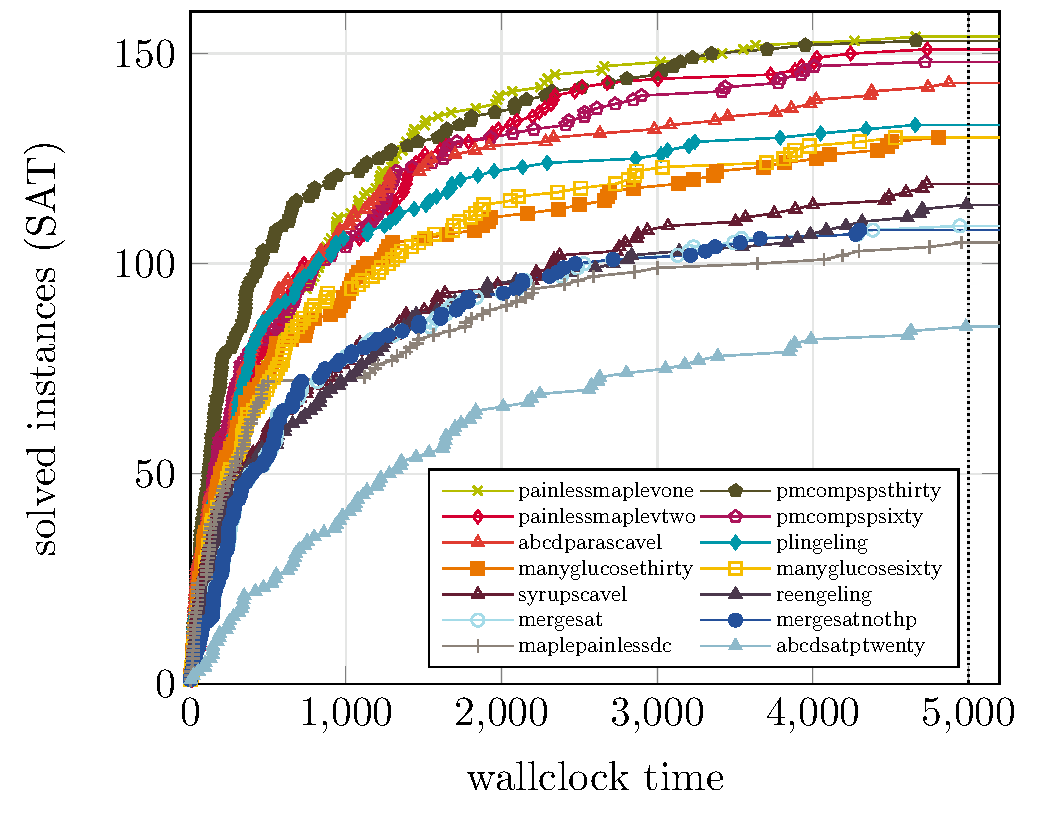
\includegraphics[width=.8\textwidth]{parallel-SAT}

\end{frame}


\begin{frame}{Parallel Track UNSAT -- Results}
The Top 3 solvers of the Parallel Track UNSAT are:
\begin{itemize}

\item[1]<4-> {\bf Plingeling} (PAR-2: 3630, 137 solved)\\
by Armin Biere
\item[2]<3-> {\bf P-MCOMSPS-STR-32} (PAR-2: 3729, 131 solved)\\
by Vincent Vallade, Ludovic Le Frioux, Souheib Baarir,\\Julien Sopena, and Fabrice Kordon

\item[3]<2-> {\bf ManyGlucose-32} (PAR-2 3844, 131 solved)\\
{\bf ManyGlucose-64} (PAR-2: 3974, 129 solved)\\
by Hidetomo Nabeshima and Katsumi Inoue
\end{itemize}
\end{frame}


\begin{frame}{Parallel Track UNSAT -- Plot}

\centering
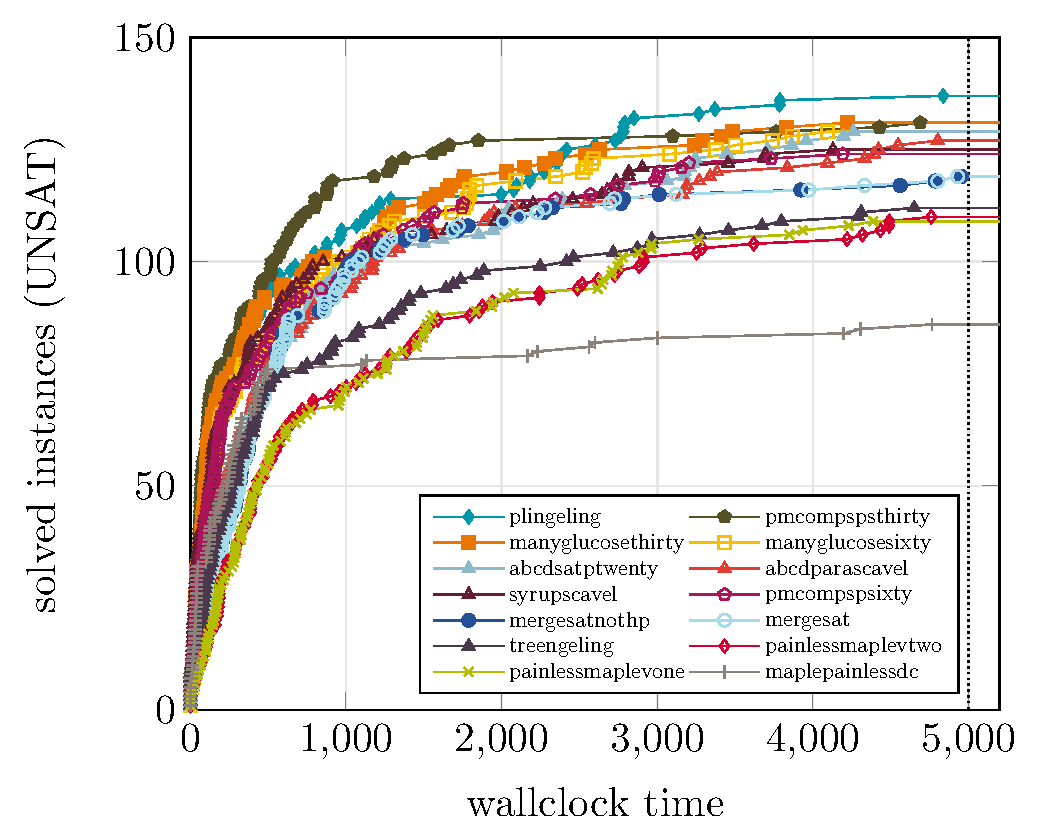
\includegraphics[width=.8\textwidth]{parallel-UNSAT}

\end{frame}

\begin{frame}{Parallel Track ALL -- Results}
The Top 3 solvers of the Parallel Track ALL are:
\begin{itemize}
\item[1]<4-> {\bf P-MCOMSPS-STR-32} (PAR-2: 3291, 284 solved)\\
{\bf P-MCOMSPS-STR-64} (PAR-2: 3689, 272 solved)\\
by Vincent Vallade, Ludovic Le Frioux, Souheib Baarir,\\Julien Sopena, and Fabrice Kordon
\item[2]<3-> {\bf Plingeling} (PAR-2: 3718, 270 solved)\\
by Armin Biere
\item[3]<2-> {\bf ManyGlucose-32} (PAR-2: 3985, 260 solved)\\
by Hidetomo Nabeshima and Katsumi Inoue
%\item[3]<2-> {\bf abcd-para-scavel} (PAR-2: 3797, 270 solved)\\
%by Zhihui Li, Guanfeng Wu, Yanh Xu, and Qingshan Chen
\end{itemize}
\end{frame}

\begin{frame}{Parallel Track ALL -- Plot}

\centering
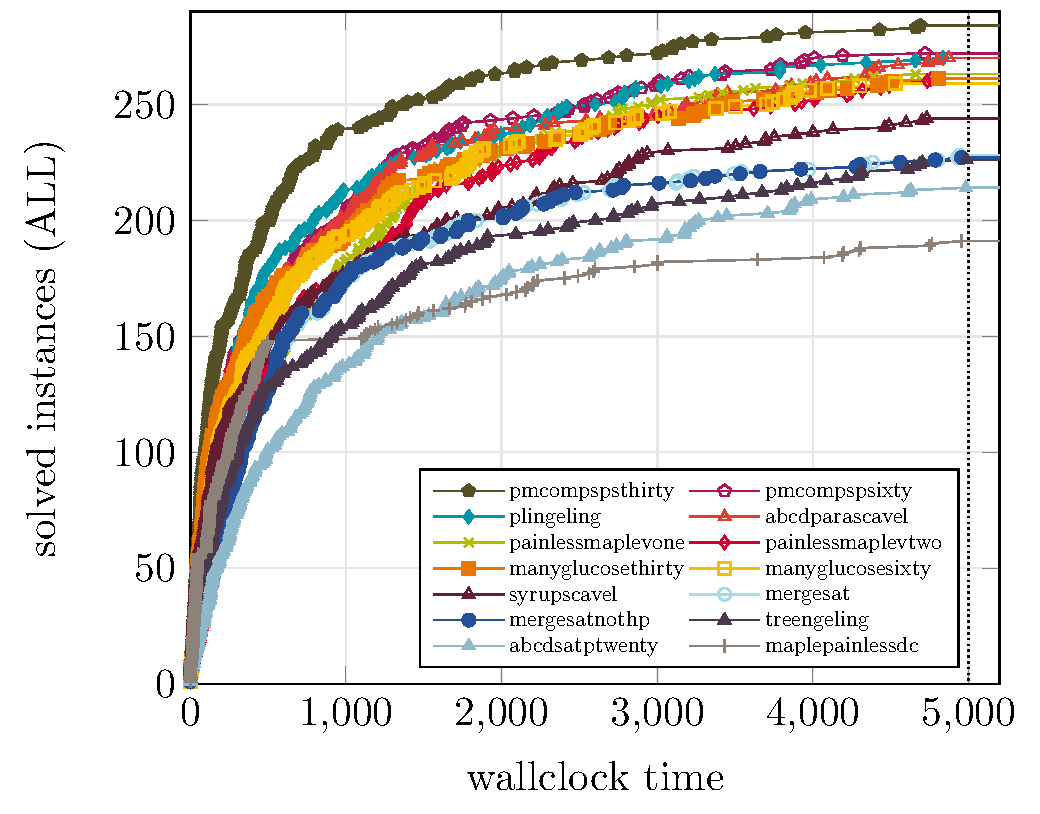
\includegraphics[width=.8\textwidth]{parallel-ALL}

\end{frame}


%%%%%%%%%%%%%%%%%%%%%%%%%%%%%%%

\begin{frame}{Cloud Track -- Results}

The Top 3 solvers of the Cloud Track are:
\begin{itemize}

\item[1]<4-> {\bf mallob-mono} (PAR-2: 2429, 306 solved)\\
by Dominik Schreiber
\item[2]<3-> {\bf TopoSAT2} (PAR-2: 3024, 283 solved)\\
by Thorsten Ehlers, Mitja Kulczynski, Dirk Nowotka, and Philipp Sieweck
\item[3]<2-> {\bf Slime} (PAR-2 4208, 239 solved)\\
by Oscar Riveros
\end{itemize}


\end{frame}

\begin{frame}{Cloud Track -- Plot}

\centering
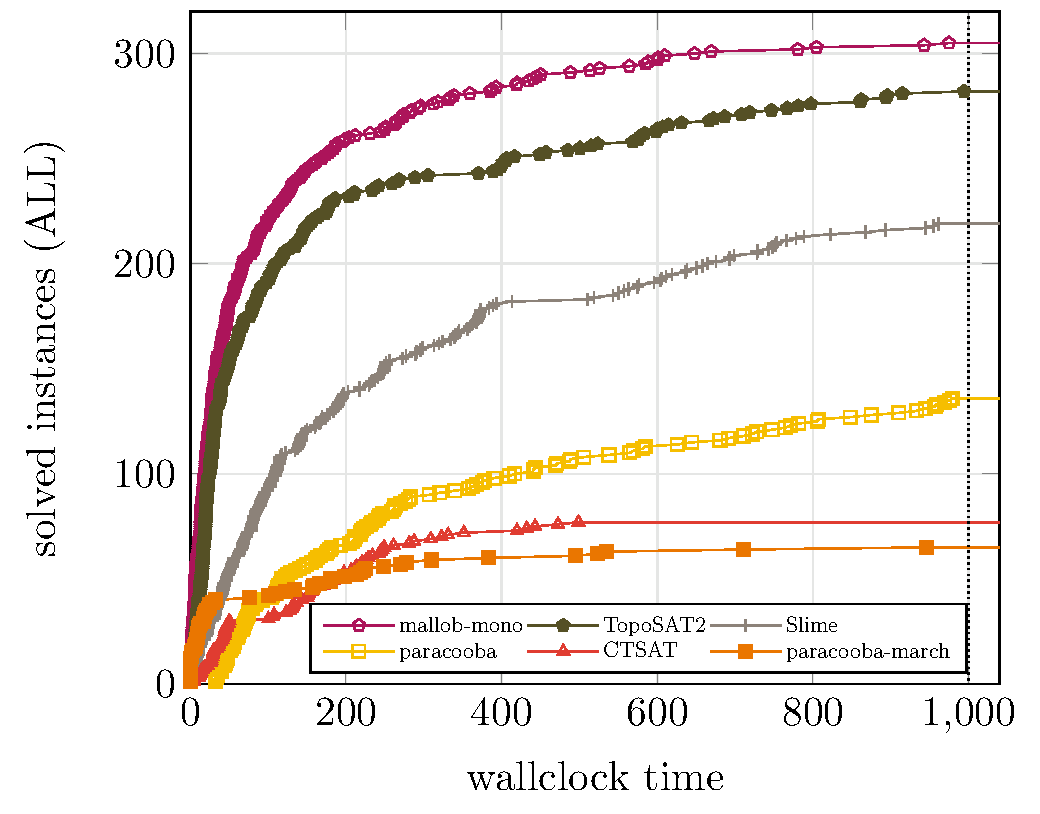
\includegraphics[width=.8\textwidth]{cloud-ALL}

\end{frame}


\begin{frame}{Main Track SAT -- Results}
The Top 3 solvers of the Main Track SAT are:
\begin{itemize}
\item[1]<4-> {\bf Relaxed\_LCMDCBDL\_newTech} (PAR-2: 2997, 150 solved)  \\
by Xindi Zhang and Shaowei Cai
\item[2]<3-> {\bf Kissat-sc2020-sat}  (PAR-2: 3128, 146 solved)\\
by Armin Biere
\item[3]<2-> {\bf Cryptominisat-ccnr-lsids} (PAR-2: 3263, 144 solved)\\
{\bf Cryptominisat-ccnr} (PAR-2: 3317, 145 solved)\\
by Mate Soos, Shaowei Cai, Jo Devriendt, Stephan Gocht,\\Arijit Shaw, and  Kuldeep Meel
\end{itemize}
\end{frame}

\begin{frame}{Main Track SAT -- Top 10 Plot}

\centering
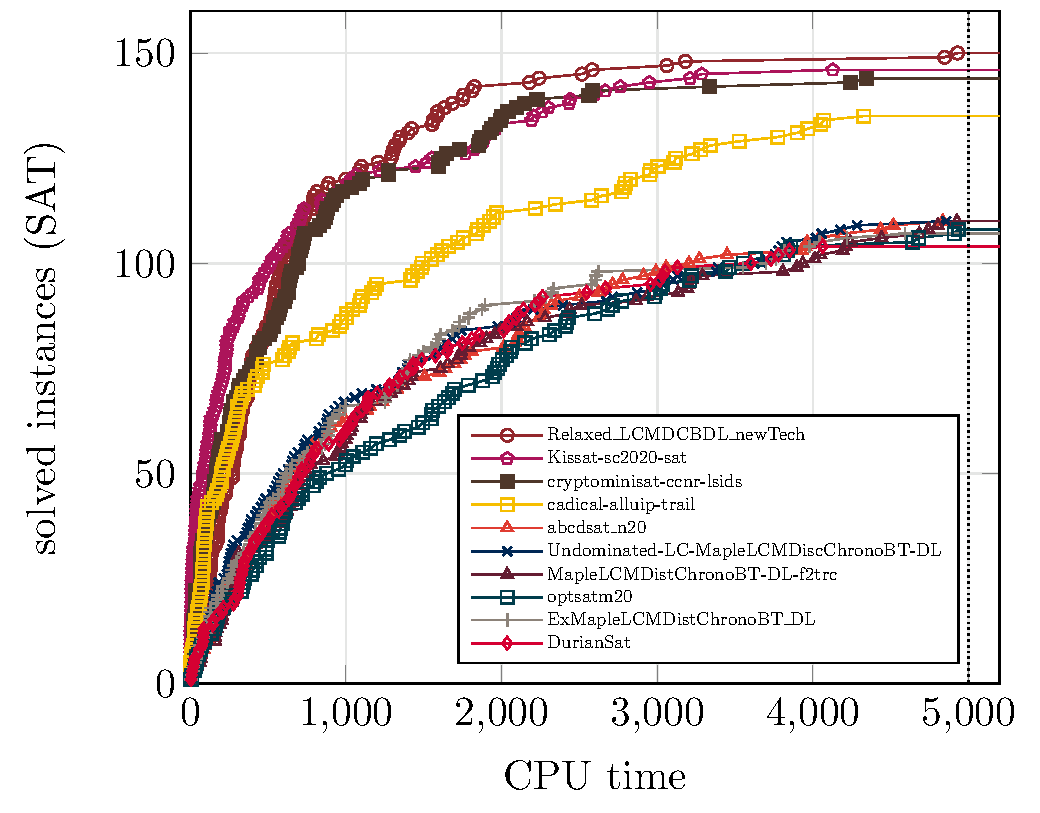
\includegraphics[width=.8\textwidth]{main-top10-SAT}

\end{frame}

\begin{frame}{Main Track UNSAT -- Results}
The Top 3 solvers of the Main Track UNSAT are:
\begin{itemize}
\item[1]<4-> 
{\bf Kissat-sc2020-unsat}  (PAR-2: 4315, 124 solved)\\
{\bf Kissat-sc2020-default}  (PAR-2: 4336, 126 solved)\\
{\bf Kissat-sc2020-sat} (PAR-2: 4725, 118 solved)\\
by Armin Biere
\item[2]<3-> {\bf CaDiCaL-trail} (PAR-2: 4842, 117 solved)\\
by Randy Hickey, Nick Feng, and Fahiem Bacchus
\item[3]<2-> {\bf MapleLCMDistChronoBT-f2trc-s} (PAR-2: 4991, 110 solved)  \\
by Stepan Kochemazov
\end{itemize}
\end{frame}


\begin{frame}{Main Track UNSAT -- Top 10 Plot}

\centering
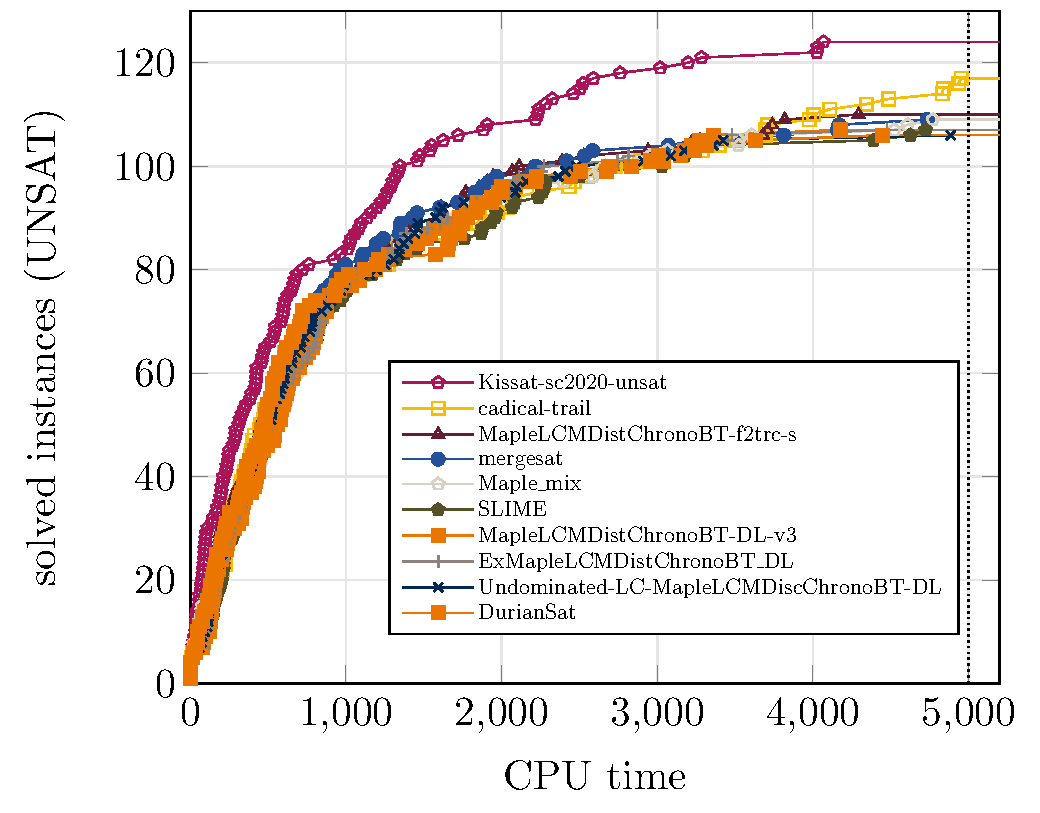
\includegraphics[width=.8\textwidth]{main-top10-UNSAT}

\end{frame}

\begin{frame}{Main Track ALL -- Results}
The Top 3 solvers of the Main Track ALL are:
\begin{itemize}
\item[1]<4-> {\bf Kissat-sc2020-sat} (PAR-2: 3926, 264 solved)\\
{\bf Kissat-sc2020-default}  (PAR-2: 4083, 260 solved)\\
by Armin Biere
\item[2]<3-> {\bf Relaxed\_LCMDCBDL\_newTech} (PAR-2: 4179, 253 solved)  \\
by Xindi Zhang and Shaowei Cai
\item[3]<2-> {\bf Cryptominisat-ccnr-lsids} (PAR-2: 4267, 248 solved)\\
{\bf Cryptominisat-ccnr} (PAR-2: 4278, 250 solved)\\
by Mate Soos, Shaowei Cai, Jo Devriendt, Stephan Gocht,\\Arijit Shaw, and  Kuldeep Meel
\end{itemize}
\end{frame}

\begin{frame}{Main Track ALL-- Top 10 Plot}

\centering
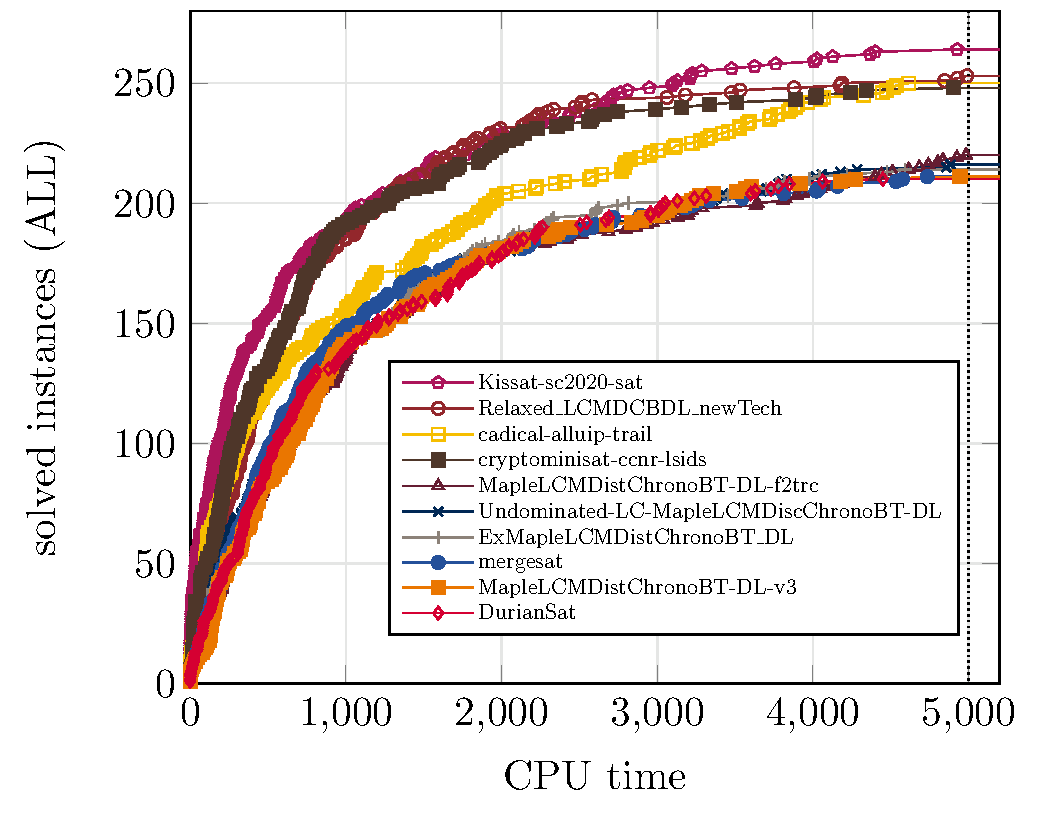
\includegraphics[width=.8\textwidth]{main-top10-ALL}

\end{frame}




\begin{frame}{More information and Acknowledgments}
Additionals Information
\begin{itemize}
	\item The Competition Proceedings (solver and benchmark descriptions)
	 will soon be available at https://satcompetition.github.io/2020/
	\item For the detailed competition results see the SAT Competition website
\end{itemize}
\medskip

Acknowledgments
\begin{itemize}
\item Thanks to all the participants
\item Thanks for all the benchmarks
\item Thanks to Mike Whalen, Jonathan Eidelman,\\and Frankie Botero at AWS
\item Thanks to Aaron Stump and StarExec
\item Thanks to CAS Software Karlsruhe for the medals
\end{itemize}
\begin{itemize}
\item Thank You for Your attention
\end{itemize}
\end{frame}


%----------------------------------------------------------------------------------------

\end{document}